\clearpage\section{Исследовательская часть}
\subsection{Условия проведения исследования}
Замеры проводились на следующей конфигурации:
\begin{itemize}
\item процессор: Intel Core i3-1115G4, 3,00 ГГц, два физических и четыре логических ядра;
\item оперативная память: 7,75 ГиБ;
\item операционная система: Windows 11;
\item компилятор: GCC 14.2.0 с флагом \texttt{-O0}.
\end{itemize}

\subsection{Методика замеров}
Для каждого сочетания размера изображения и числа потоков выполнялось 100 повторений, после чего вычислялось среднее арифметическое. Реальное время полного расчёта измерялось с помощью QueryPerformanceCounter~\cite{timer}. Создание, синхронизация и завершение рабочих потоков учитывались; генерация изображения и файловый ввод-вывод в замер не включались.

Использовались квадратные полутоновые изображения со сторонами 256, 512, 1024, 2048 и 4096 пикселей. Для каждого размера обеим версиям передавалось одно и то же изображение. Число рабочих потоков $q\in\{1,2,4,8,16,32\}$ соответствует диапазону от одного до $8\cdot k$, где $k=4$ --- число логических ядер. Помимо параллельной версии при одном рабочем потоке отдельно измерялась последовательная версия.

\subsection{Результаты замеров}
В таблице~\ref{tab:sizes} представлены средние времена последовательной версии и параллельной версии при одном рабочем потоке.
\begin{table}[H]\caption{Сравнение реализаций при разных размерах}\label{tab:sizes}
\centering\begin{tabularx}{\textwidth}{|c|X|X|}\hline
Сторона, пиксель & Послед., мс & Паралл., $q=1$, мс\\\hhline{|=:=:=|}
256 & 0,186 & 0,401 \\\hline
512 & 0,701 & 1,075 \\\hline
1024 & 3,538 & 4,900 \\\hline
2048 & 34,857 & 46,870 \\\hline
4096 & 132,034 & 173,095 \\\hline
\end{tabularx}\end{table}

На рисунке~\ref{fig:time} представлена зависимость времени от размера изображения для всех исследованных конфигураций. Обе оси имеют логарифмический масштаб.
\begin{figure}[H]\centering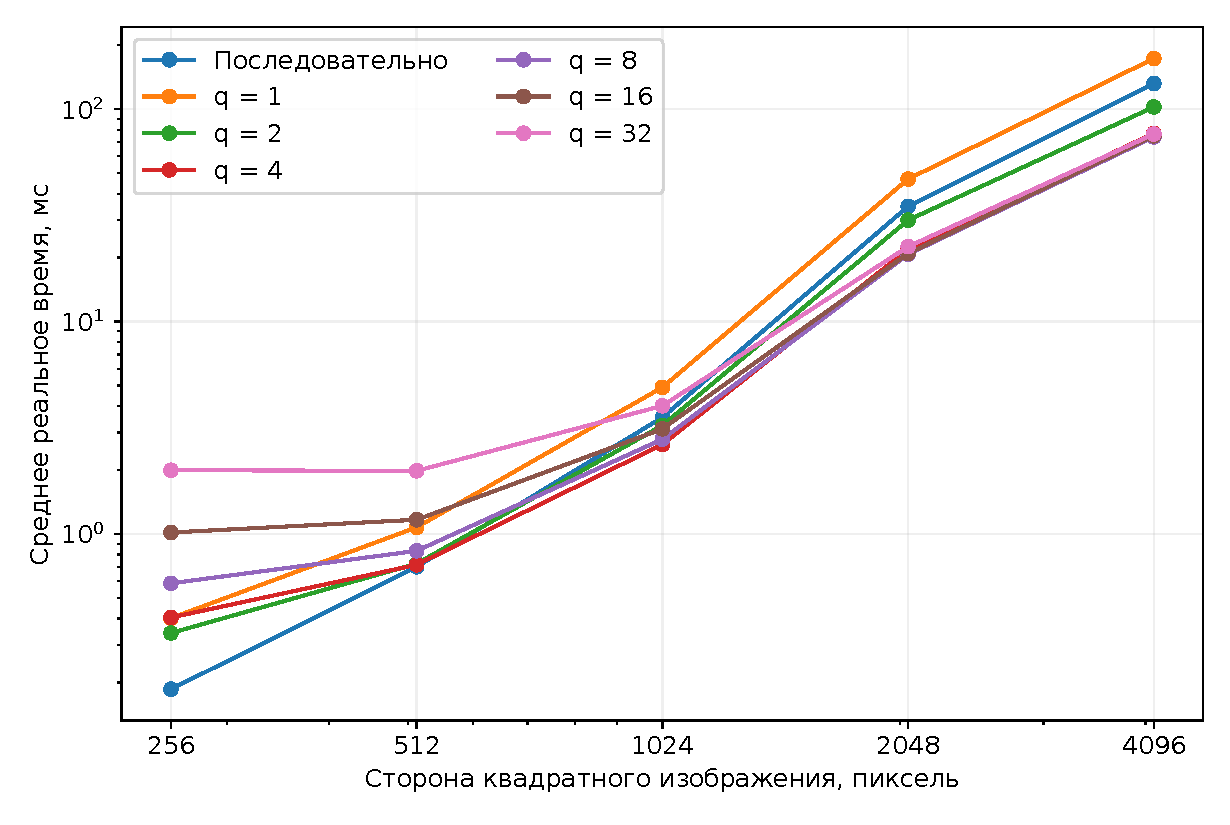
\includegraphics[width=\textwidth]{figures/time.pdf}
\caption{Зависимость среднего реального времени от размера изображения}\label{fig:time}\end{figure}

Для изображения $4096\times4096$ результаты при разном числе рабочих потоков приведены в таблице~\ref{tab:q}. Ускорение рассчитывается как отношение среднего времени последовательной версии к среднему времени параллельной версии. Полные результаты приведены в приложении~Б.
\begin{table}[H]\caption{Результаты для изображения $4096\times4096$}\label{tab:q}
\centering\begin{tabularx}{\textwidth}{|c|X|X|}\hline
Рабочие потоки & Время, мс & Ускорение\\\hhline{|=:=:=|}
1 & 173,095 & 0,76 \\\hline
2 & 102,399 & 1,29 \\\hline
4 & 76,934 & 1,72 \\\hline
8 & 73,955 & 1,79 \\\hline
16 & 74,901 & 1,76 \\\hline
32 & 76,335 & 1,73 \\\hline
\end{tabularx}\end{table}

На рисунке~\ref{fig:speedup} представлена зависимость ускорения от числа рабочих потоков. Значения меньше единицы соответствуют замедлению.
\begin{figure}[H]\centering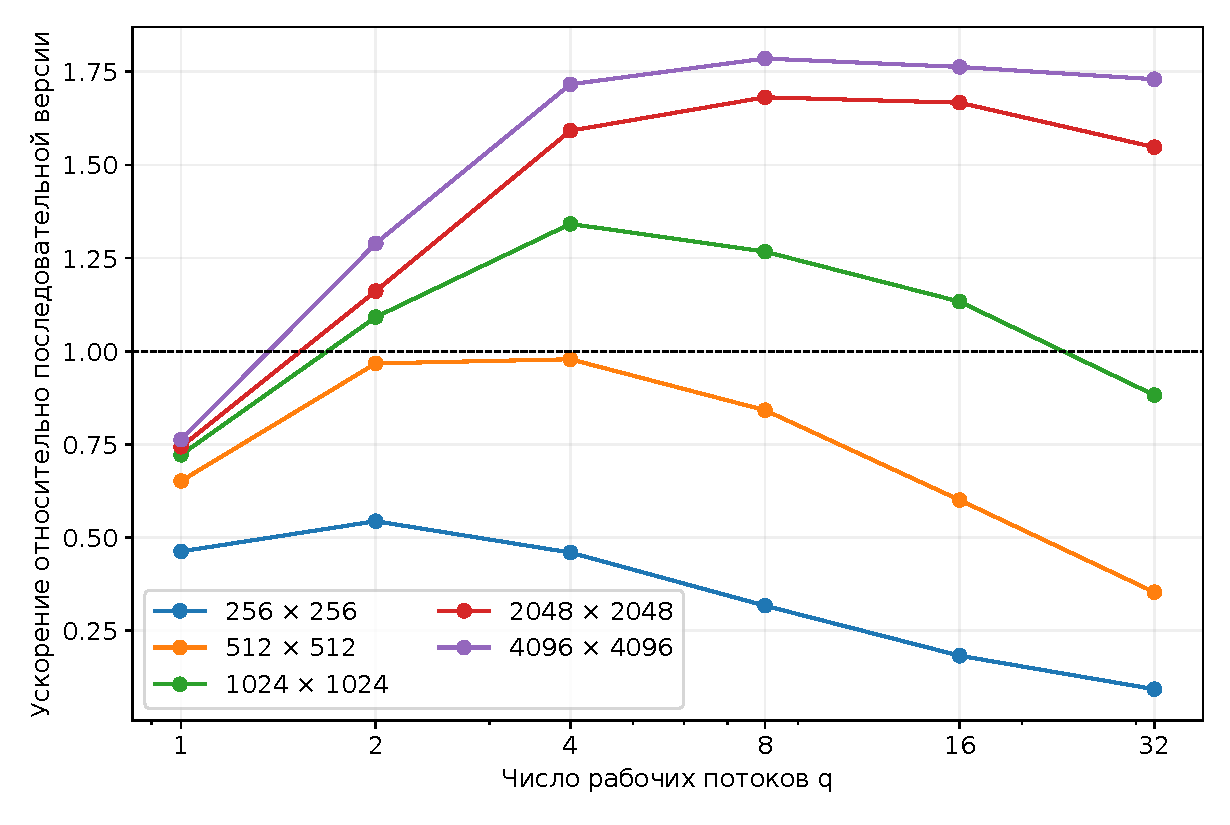
\includegraphics[width=\textwidth]{figures/speedup.pdf}
\caption{Ускорение параллельной реализации при разных размерах}\label{fig:speedup}\end{figure}

\subsection{Анализ результатов}
На изображениях $256\times256$ и $512\times512$ параллельная версия не дала выигрыша: расходы на управление потоками превышают сокращение времени обработки пикселей. Начиная с $1024\times1024$ в исследованном наборе получено ускорение при нескольких рабочих потоках.

При одном рабочем потоке параллельная версия медленнее последовательной для всех размеров. Для $4096\times4096$ время увеличилось с 132,034 до 173,095 мс, то есть примерно на 31\,\%.

Для наибольшего изображения минимальное среднее время получено при восьми рабочих потоках: 73,955 мс, ускорение 1,79. Дальнейшее увеличение числа потоков заметного выигрыша не дало. Результаты при 4, 8, 16 и 32 потоках близки с учётом разброса измерений, поэтому устойчивое преимущество восьми потоков не утверждается. Замеры выполнялись в обычной настольной среде без фиксации частоты процессора.
